\newpage

\section{Otimization Objective}


\quad In the process of optimization, we undertook the following steps to improve our approach:\\


Initially, we developed an evaluation function based on the statement provided by the professor. This function served as the foundation for our optimization efforts. However, we soon realized that our initial implementation was not aligned with sound software engineering practices.\\


To address this, we decided to refactor the function. Our primary objective was to introduce flexibility by allowing the specification of the number of days to evaluate. Unfortunately, due to the nature of the input, we were always limited to 7 days.\\


What set our implementation apart from others was our approach to reducing the number of variables. We concluded that since most algorithms generated values randomly, we could streamline the process by utilizing only six variables. These variables, namely bud v1, bud v2, bud v3, stella v1, stella v2, and stella v3, represented the quantities of beer per brand allocated to different resources \(v1, v2, v3\). We found no constraints in the provided statement that prohibited placing different beer brands within the same resource.\\


By leveraging this reduced set of variables, we were able to infer the remaining values based on the output generated by the respective algorithms. The analogy of playing dominoes accurately describes this approach, as each value falls into place based on the preceding one.\\


This methodology significantly minimized the need for value repairs. 
Since the values were inferred in accordance with the algorithm's output, we encountered fewer instances where, for instance, there were 100 beers in v1 resource but none in storage—a highly improbable scenario.\\


Furthermore, we established that a value range of 0 to 100 was suitable for the resources. Given that the total quantity of beers did not exceed 200, this range provided a reasonable and logical representation. Additionally, it allowed for sending a maximum of 300 units in a single day per resource, which surpassed practical requirements. By adhering to this range, the randomly generated values aligned with our expectations, ensuring meaningful results.\\


Initially, our focus revolved around maximizing profits, which required optimizing the entire function. To achieve this, we employed various algorithms, including hill climbing and Monte Carlo simulation.\\


As we shifted our attention towards minimizing the costs, we explored additional algorithms such as simulated annealing, SANN, grid search, and tabu search. However, after thorough evaluation, we concluded that Monte Carlo simulation and hill climbing emerged as the most effective algorithms for our specific problem. The alternative approaches failed to produce satisfactory results when evaluated against our optimization objectives.\\



This report extends the analysis of the Hill Climbing and Monte Carlo algorithms' performance for beer production optimization by comparing the optimal results achieved in Week 3 and Week 20. The focus is on identifying the best outcomes in terms of production predictions and evaluation scores for each algorithm in these two weeks.\\

Week 3 Analysis:\\

In Week 3, both the Hill Climbing and Monte Carlo algorithms were subjected to 2000 iterations. The optimal results obtained by each algorithm are as follows:\\

\quad Hill Climbing:

\quad \quad \textbullet Stella Prevision: 119, 167, 119, 91, 85, 55;

\quad \quad \textbullet Bud Prevision: 62, 73, 74, 50, 76, 39;

\quad \quad \textbullet Evaluation Score: 3879.2.\\

\quad Monte Carlo:

\quad \quad \textbullet Stella Prevision: 119, 167, 119, 91, 85, 55;

\quad \quad \textbullet Stella Prevision: 119, 167, 119, 91, 85, 55;

\quad \quad \textbullet Bud Prevision: 62, 73, 74, 50, 76, 39;

\quad \quad \textbullet Evaluation Score: 3676.1.\\

Comparing the algorithms, it is evident that both Hill Climbing and Monte Carlo produced identical predictions for Stella and Bud beer production in Week 3. However, the evaluation score favored the Monte Carlo algorithm, indicating its superior performance in optimizing the production levels during this week.\\



\begin{figure}[H]
    \centering
    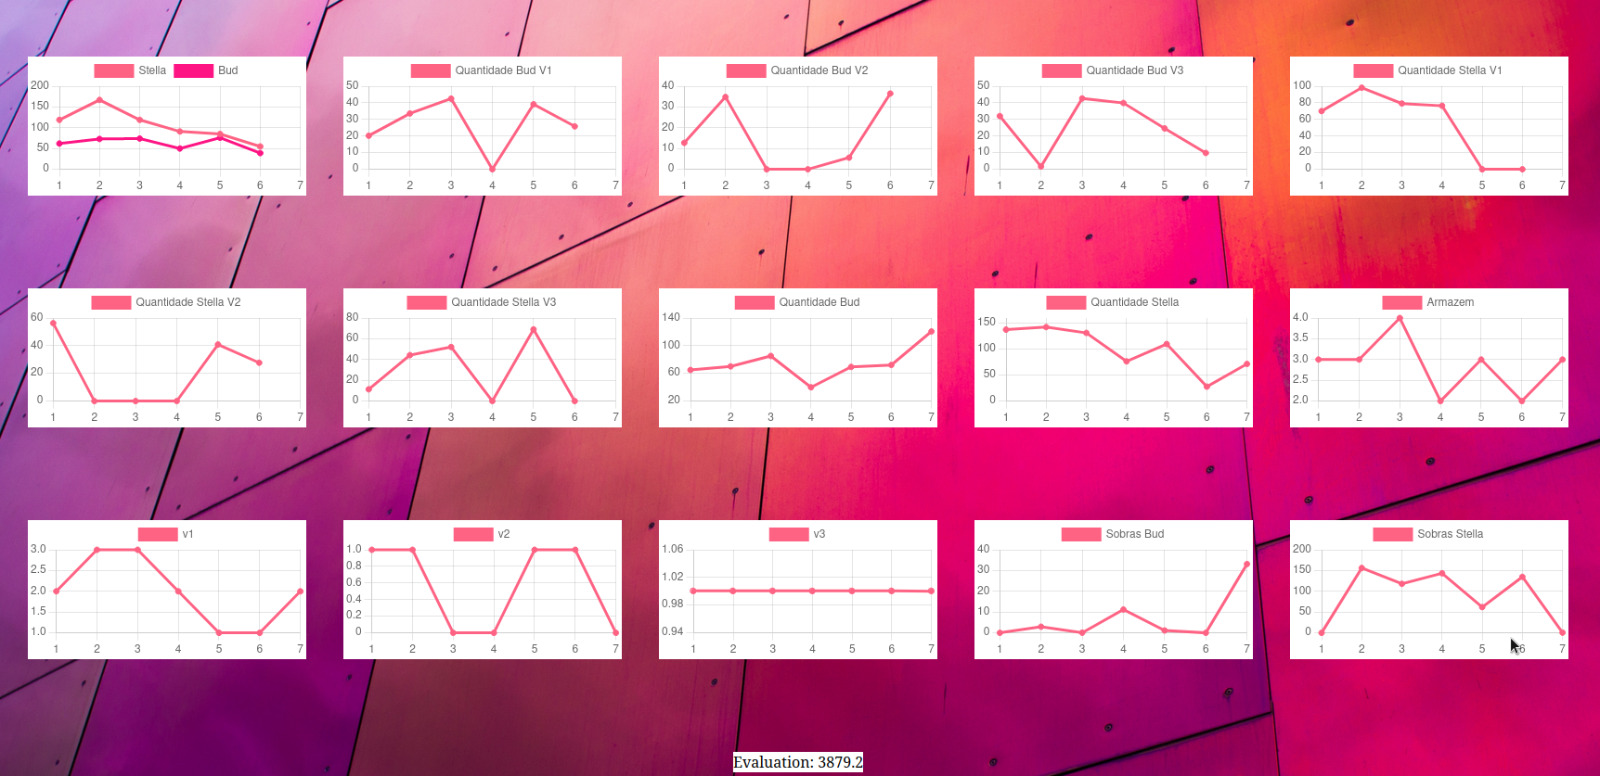
\includegraphics[width=1\textwidth]{assets/oo1.jpeg}
    \caption{Multivariate Analysis}
    \label{fig:mulivariate_dataset}
    \end{figure}


\begin{figure}[H]
    \centering
    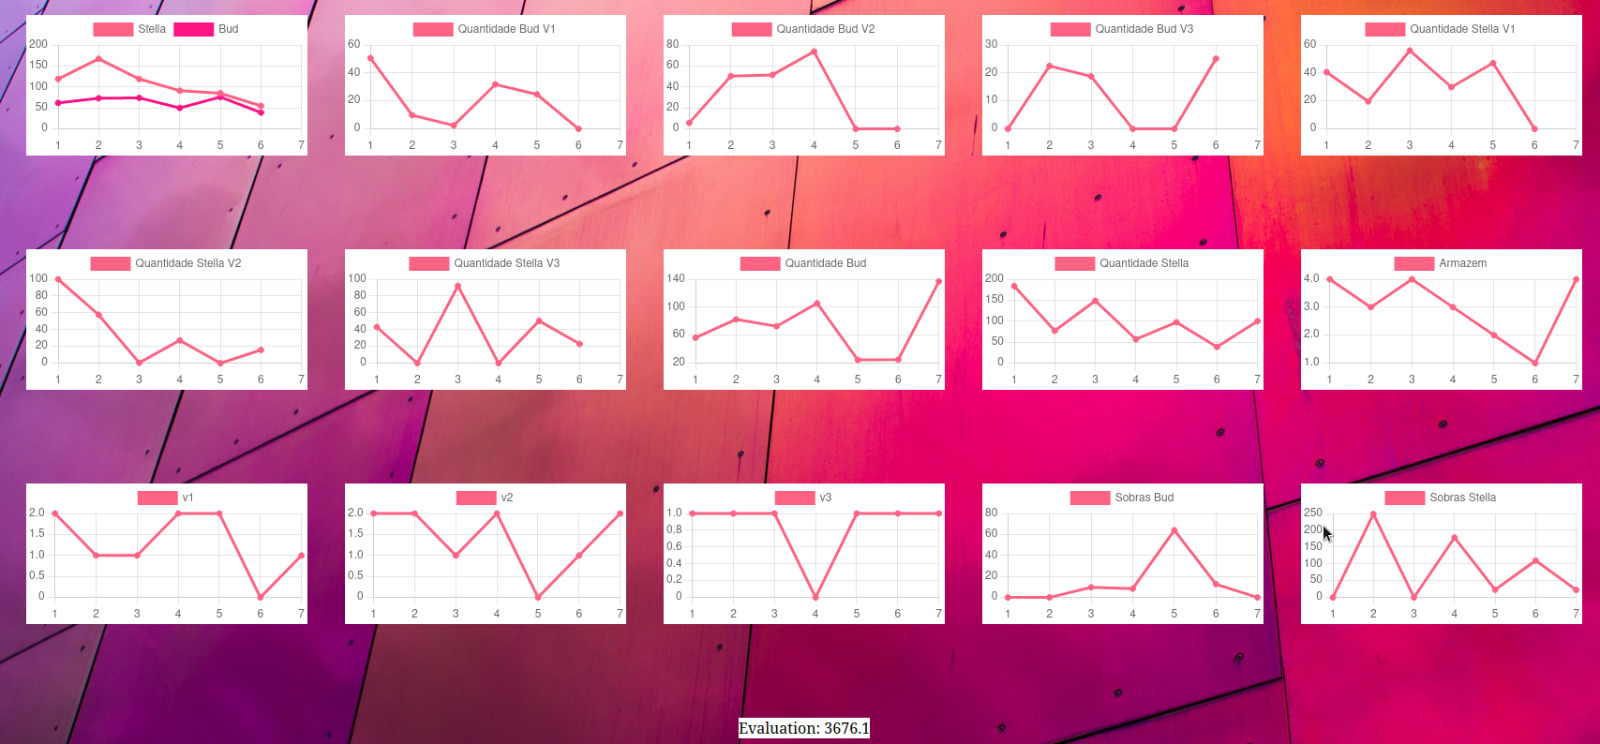
\includegraphics[width=1\textwidth]{assets/oo2.jpeg}
    \caption{Multivariate Analysis}
    \label{fig:mulivariate_dataset}
    \end{figure}



Week 20 Analysis:\\

In Week 20, once again using 2000 iterations, the algorithms' optimal results were as follows:

\quad Hill Climbing:

\quad \quad \textbullet Stella Prevision: 84, 137, 127, 145, 109, 89;

\quad \quad \textbullet Bud Prevision: 115, 234, 243, 154, 207, 132;

\quad \quad \textbullet Evaluation Score: 8471.8.\\

\quad Monte Carlo:

\quad \quad \textbullet Stella Prevision: 84, 137, 127, 145, 109, 89;

\quad \quad \textbullet Bud Prevision: 115, 234, 243, 154, 207, 132;

\quad \quad \textbullet Evaluation Score: 8518.1.\\

Analyzing the optimal results in Week 20, both algorithms once again produced similar predictions for Stella and Bud beer production. However, the evaluation scores indicate a marginal advantage for the Monte Carlo algorithm, suggesting its slightly better performance in optimizing production levels during this week.




\begin{figure}[H]
    \centering
    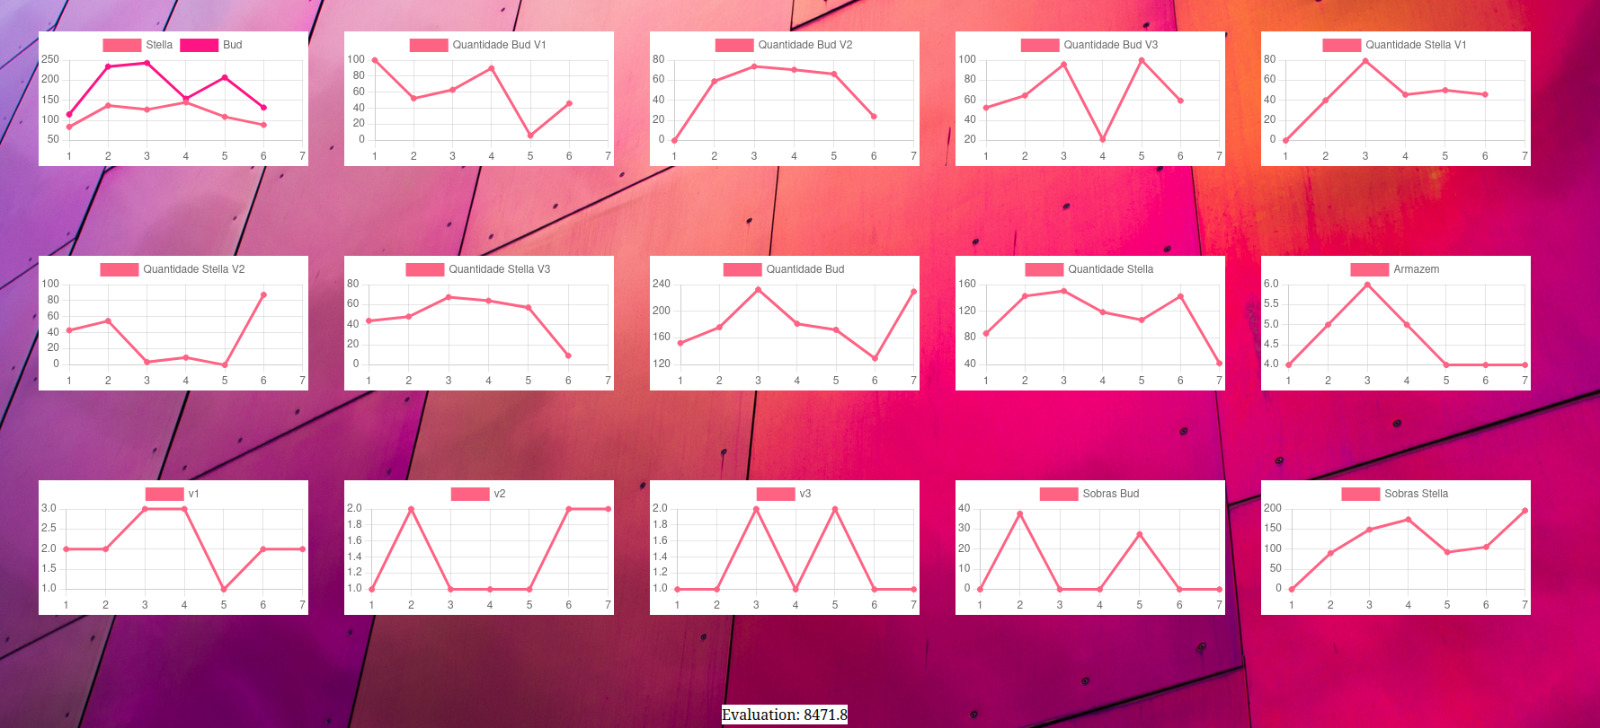
\includegraphics[width=1\textwidth]{assets/oo3.jpeg}
    \caption{Multivariate Analysis}
    \label{fig:mulivariate_dataset}
    \end{figure}


\begin{figure}[H]
    \centering
    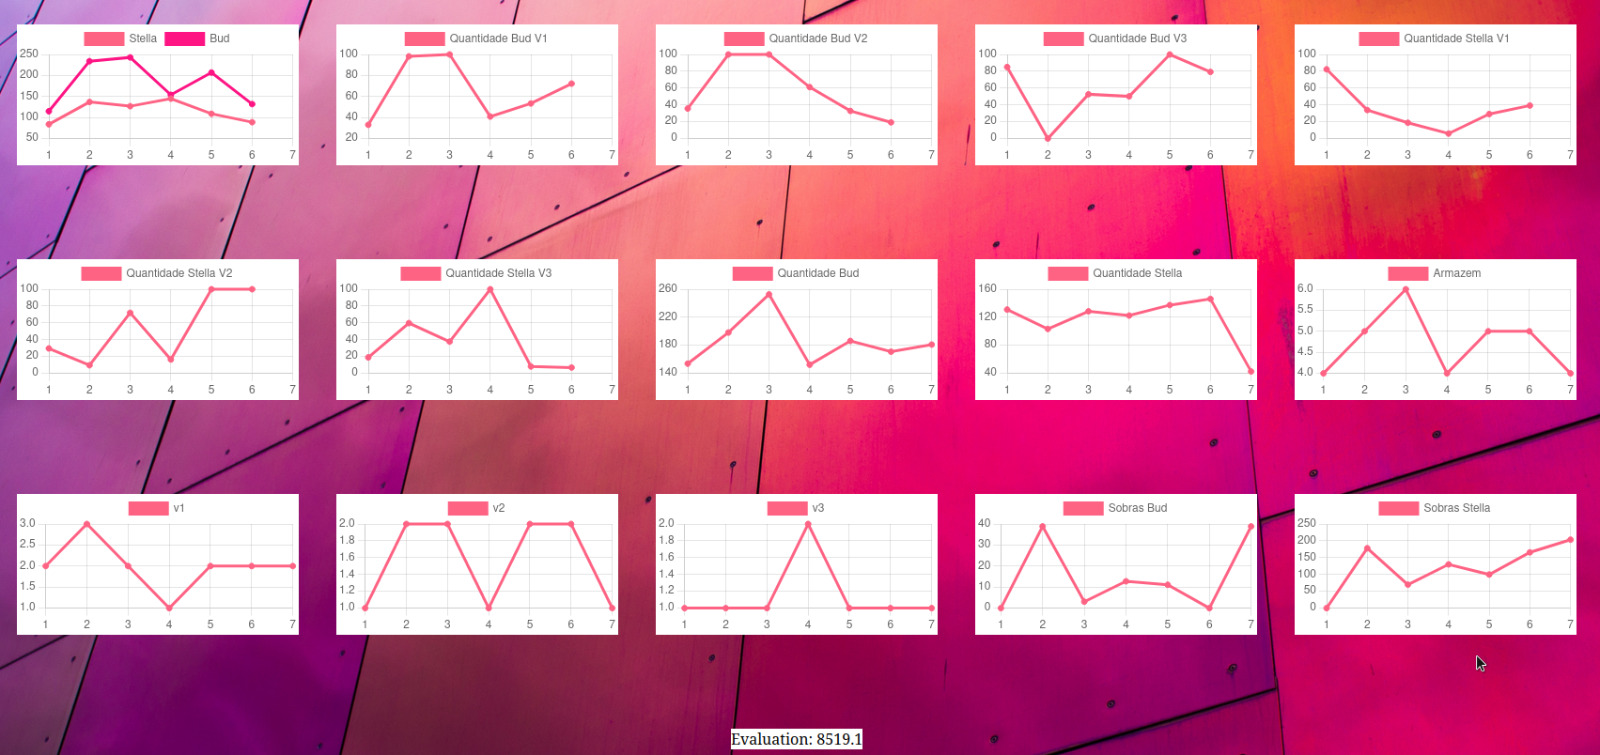
\includegraphics[width=1\textwidth]{assets/oo4.jpeg}
    \caption{Multivariate Analysis}
    \label{fig:mulivariate_dataset}
    \end{figure}



Comparison between Weeks 3 and 20:\\

Comparing the best results achieved by each algorithm in Weeks 3 and 20, the following observations can be made:\\

\textbullet Hill Climbing: In terms of production predictions, Hill Climbing maintained the same predictions for Stella and Bud beer production in both weeks. However, the evaluation score was higher in Week 20 (8471.8) compared to Week 3 (3879.2), indicating improved optimization in the latter week.\\

\textbullet Monte Carlo: The Monte Carlo algorithm also maintained consistent production predictions for Stella and Bud beer in both weeks. However, the evaluation score was higher in Week 20 (8518.1) compared to Week 3 (3676.1), indicating better overall optimization in the latter week.\\
    
The comparison of optimal results achieved by the Hill Climbing and Monte Carlo algorithms in Weeks 3 and 20 highlights interesting insights. Both algorithms produced similar predictions for beer production in both weeks, but the evaluation scores demonstrated a preference for the Monte Carlo algorithm. It achieved slightly higher scores in both weeks, indicating better overall performance in optimizing production levels. Further analysis and experimentation are recommended to understand the strengths and weaknesses of these algorithms for beer production optimization across different time periods and evaluate their suitability for real-world brewery operations.